\section{Il progetto \ProjectTitle}

    % Griglia con le 4 immagini della presentazione
    \begin{figure}[H]
        \begin{subfigure}{0.5\textwidth}
            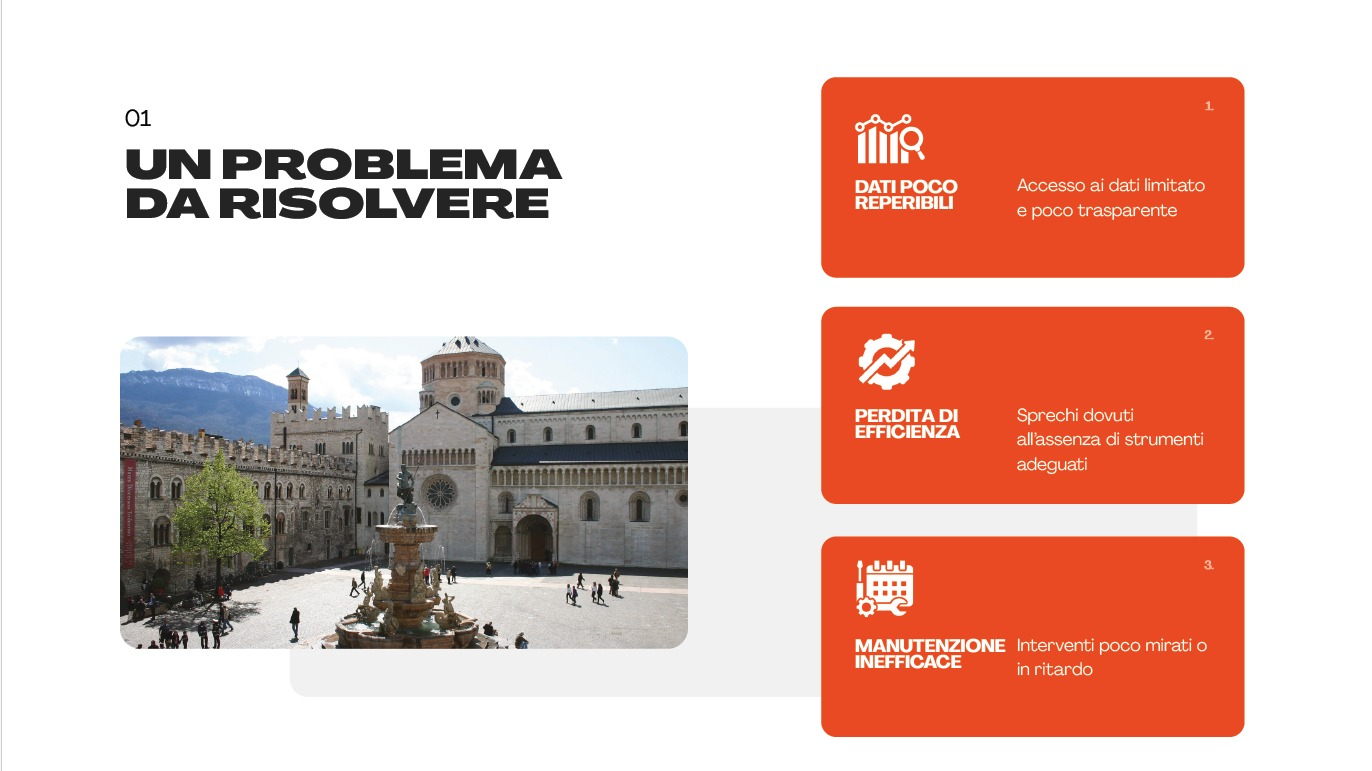
\includegraphics[width=\textwidth]{../images/Slides/Slide_1.jpeg}
        \end{subfigure}
        \begin{subfigure}{0.5\textwidth}
            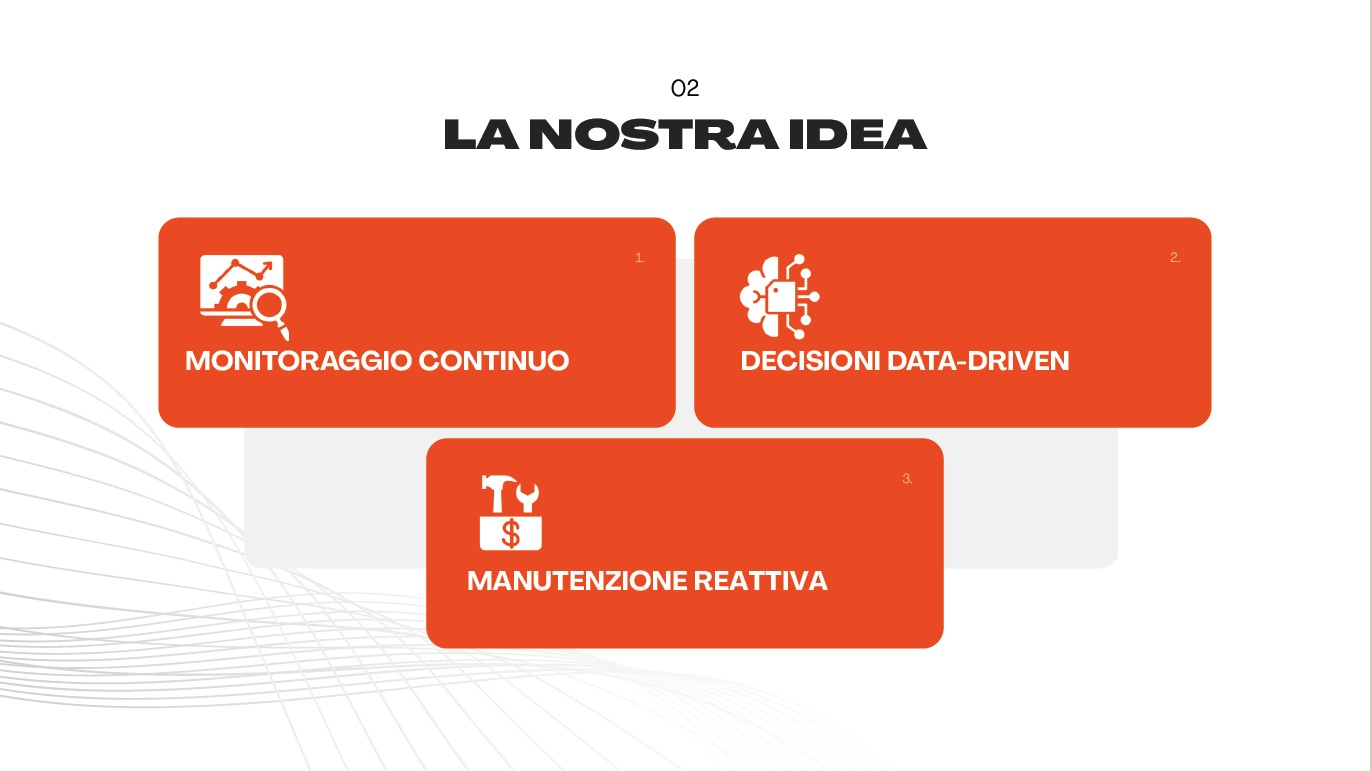
\includegraphics[width=\textwidth]{../images/Slides/Slide_2.jpeg}
        \end{subfigure}
        \begin{subfigure}{0.5\textwidth}
            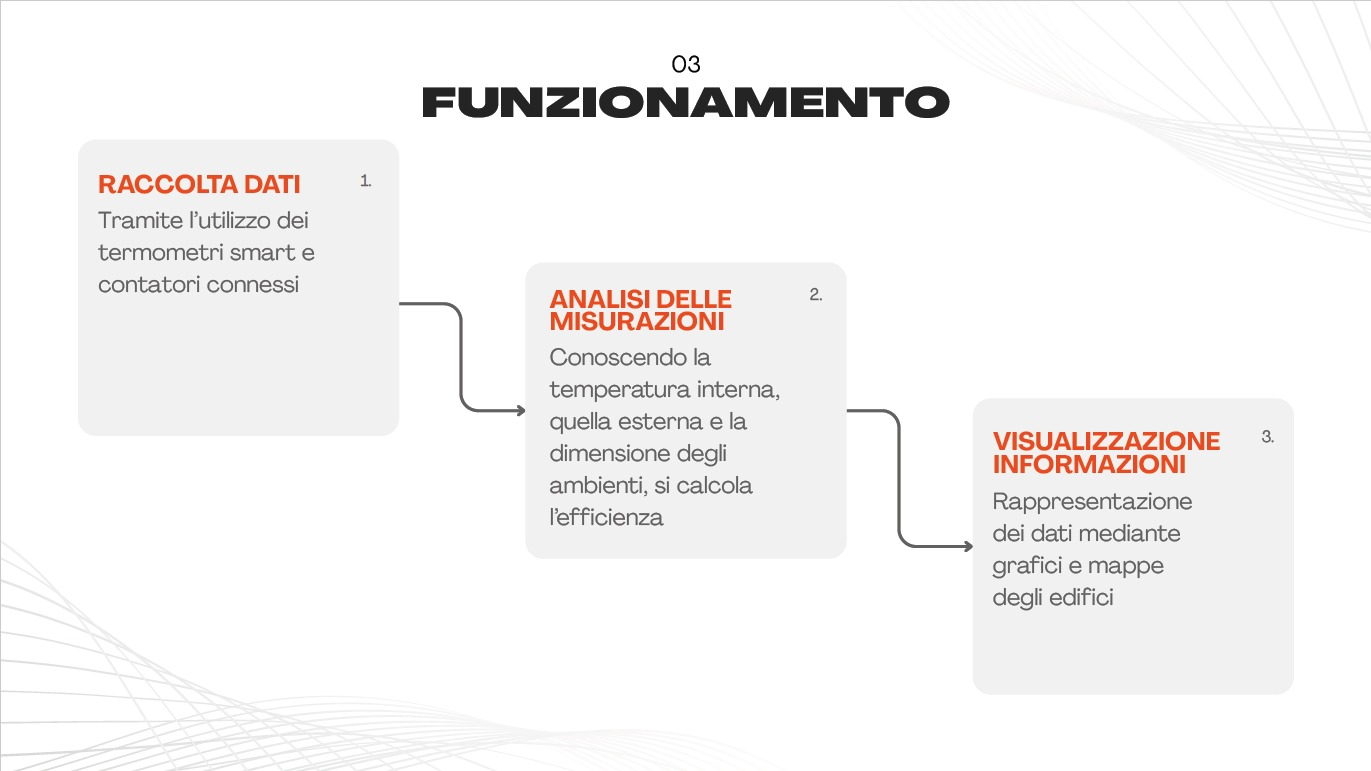
\includegraphics[width=\textwidth]{../images/Slides/Slide_3.jpeg}
        \end{subfigure}
        \begin{subfigure}{0.5\textwidth}
            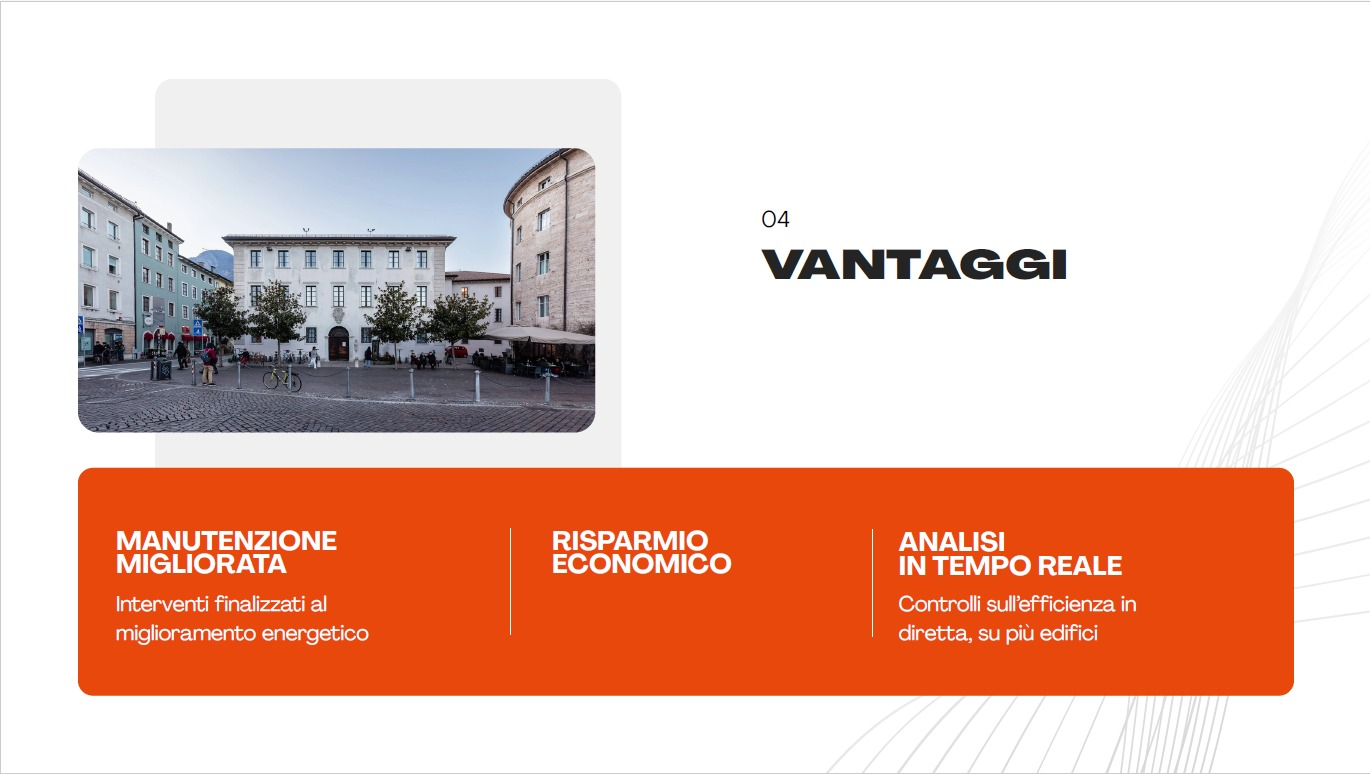
\includegraphics[width=\textwidth]{../images/Slides/Slide_4.jpeg}
        \end{subfigure}
    \end{figure}

\subsection{I problemi}
Il progetto mira a risolvere le criticità legate al monitoraggio dei consumi e allo spreco energetico causato dagli impianti di riscaldamento degli edifici pubblici del Comune di Trento. \newline
Il primo problema riguarda la limitata reperibilità dei dati poiché attualmente non esiste un sistema centralizzato e accessibile online che consenta una gestione digitale di queste informazioni. Senza una visione d'insieme, gli amministratori comunali e i tecnici faticano a individuare sprechi e anomalie. \newline
Il secondo problema è l'assenza di un monitoraggio in tempo reale; questo comporta l'incapacità di rilevare immediatamente malfunzionamenti dei termometri o cali di efficienza energetica. Questa mancanza si tramuta in manutenzioni reattive, costi elevati e un notevole spreco di risorse economiche e termiche. \newline
L'ultimo problema consiste nella mancanza di chiarezza dei dati energetici a disposizione dei cittadini e degli uffici tecnici. Attualmente non esiste un'applicazione accessibile per l'analisi dei parametri termici e dei consumi; questa mancanza penalizza la capacità di prendere scelte consapevoli
\subsection{La soluzione}
Il progetto WattGuard realizza un'applicazione web fruibile tramite browser, senza necessità di installare software aggiuntivi. Tale applicazione permette di monitorare in tempo reale i consumi energetici e le temperature di ogni edificio pubblico. \newline
I dati vengono acquisiti tramite termometri intelligenti collegati via Internet e contatori di consumo, integrati con API meteo per rilevare la temperatura esterna. Questi dati vengono elaborati e visualizzati sotto forma di cruscotti (dashboard), grafici storici e mappe interattive. \newline
L'applicazione offre funzionalità avanzate come le notifiche automatiche in caso di anomalie, cali di prestazioni o malfunzionamenti, in modo da facilitare una manutenzione reattiva. Inoltre, il sistema garantisce la massima conformità alle normative sulla protezione dei dati personali (GDPR) e l'accesso differenziato in base ai ruoli (Amministratore e Operatore Tecnico).

\subsection{I vantaggi}
\begin{itemize}
    \item \textbf{Manutenzione migliorata:} L'integrazione di termometri smart permette un monitoraggio continuo e accurato delle condizioni termiche, individuando tempestivamente eventuali anomalie e riducendo i tempi di intervento.
    \item \textbf{Risparmio economico:} L'analisi costante dei dati consente di ottimizzare l'utilizzo delle risorse e identificare sprechi energetici, portando a una riduzione delle bollette e dei costi di gestione.
    \item \textbf{Analisi in tempo reale:} La piattaforma permette la raccolta, elaborazione e visualizzazione in tempo reale di parametri termici e prestazioni energetiche, garantendo una visione sempre aggiornata dello stato degli impianti.
    \item \textbf{Conformità e Sicurezza:} Il sistema garantisce la gestione protetta dei dati personali e rispetta le normative vigenti in materia di protezione dei dati, offrendo un ambiente sicuro per gli operatori e gli amministratori.
\end{itemize}

\subsection{Limiti dell'applicazione}
\begin{itemize}
    \item \textbf{Margine di incertezza nella stima dell’efficienza energetica:} L’applicazione elabora i dati raccolti dai termometri smart per stimare l’efficienza energetica degli impianti. Tuttavia, tali stime possono essere influenzate da diverse variabili esterne (come condizioni ambientali, la calibrazione dei sensori, le differenze di installazione o i comportamenti d’uso non monitorati). Di conseguenza, i risultati ottenuti non sempre rappresentano una misurazione diretta e assoluta dell’efficienza, ma piuttosto una valutazione indicativa utile a individuare tendenze, anomalie o potenziali aree di miglioramento.
    \item \textbf{Dipendenza da una connessione internet:} Il corretto funzionamento dell’applicazione richiede una connessione stabile e sicura tra i termometri smart e la piattaforma web. Eventuali problematiche infrastrutturali (ad esempio in aree con segnale debole o reti datate) potrebbero compromettere la raccolta continua dei dati o introdurre ritardi nelle analisi in tempo reale.
    \item \textbf{Costi implementativi e Manutenzione tecnologica:} L’adozione di termometri e contatori smart, oltre all’integrazione con una piattaforma digitale, comporta investimenti iniziali significativi, legati sia all’acquisto dei dispositivi sia allo sviluppo e alla manutenzione del software. Nel lungo periodo, sarà necessario prevedere risorse per l’aggiornamento dei sistemi, la calibrazione dei sensori e l’assistenza tecnica.
\end{itemize}